\section{Wyniki pomiarów działania programu}
\subsection{Dokładność modeli w bazie}
Badania przeprowadzono dla różnych liczb n-literowych końcówek wyrazów. 
\begin{landscape}
	\noindent Aby lepiej zobrazować otrzymane wyniki użyto notacji:\\ (liczba 1 literowych końcówek, liczba 2 literowych końcówek, liczba 3 literowych końcówek, liczba 4 literowych końcówek).
	\begin{table}[!htbp]
		\centering
		\caption{Skuteczność modeli -- Korpus PWr.}
		\begin{tabular}{cccccccc}
			\toprule
			\textbf{Algorytm} & \textbf{(15, 35, 35, 35)} & \textbf{(20, 35, 35, 35)} & \textbf{(25, 38, 38, 38)} & \textbf{(25, 40, 40, 40)} & \textbf{(28, 42, 42, 42)} & \textbf{(28, 45, 45, 45)} & \textbf{(32, 45, 45, 45)} \\
			\midrule
			Support Vector Machine & 56,46 & 57,46 & 58,75 & 60,03 & 61,01 & 59,94 & 58,68 \\
			Decision Trees & 57,24 & 58,12 & 59,30 & 59,97 & 60,58 & 59,10 & 58,14 \\
			Stochastic Gradient Descent & 53,62 & 54,48 & 55,37 & 56,58 & 57,72 & 56,22 & 54,97 \\
			Logistic Regression & 55,57 & 56,68 & 57,93 & 58,82 & 59,93 & 58,79 & 57,84 \\
			Naive Bayes & 54,14 & 55,42 & 56,69 & 57,72 & 58,89 & 57,58 & 56,56 \\
			K Neighbors & 50,17 & 51,35 & 52,18 & 53,30 & 54,22 & 53,12 & 52,20 \\
			Neural Networks & 55,80 & 57,08 & 57,91 & 58,88 & 60,04 & 58,72 & 57,75 \\ 
			Klasyfikator GPU & 56,24 & 57,46 & 58,34 & 59,23 & 60,51 & 59,1 & 58,22 \\
			\bottomrule
		\end{tabular}
	\end{table}
	
	\begin{table}[!htbp]
		\centering
		\caption{Skuteczność modeli -- korpus National.}
		\begin{tabular}{cccccccc}
			\toprule
			\textbf{Algorytm} & \textbf{(15, 35, 35, 35)} & \textbf{(20, 35, 35, 35)} & \textbf{(25, 38, 38, 38)} & \textbf{(25, 40, 40, 40)} & \textbf{(28, 42, 42, 42)} & \textbf{(28, 45, 45, 45)} & \textbf{(32, 45, 45, 45)} \\
			\midrule
			Support Vector Machine & 55,43 & 56,26 & 57,63 & 59,05 & 60,13 & 59,07 & 57,55 \\
			Decision Trees & 56,04 & 57,03 & 58,25 & 59,10 & 59,38 & 57,97 & 57,15 \\
			Stochastic Gradient Descent & 53,56 & 54,35 & 55,30 & 56,53 & 57,62 & 56,16 & 54,85 \\
			Logistic Regression & 55,48 & 56,55 & 57,82 & 58,76 & 59,86 & 58,64 & 57,77 \\
			Naive Bayes & 53,11 & 54,28 & 55,70 & 56,61 & 58,06 & 56,59 & 55,39 \\
			K Neighbors & 50,02 & 51,29 & 52,03 & 53,25 & 54,13 & 53,00 & 52,08 \\
			Neural Networks & 54,69 & 56,17 & 56,95 & 57,81 & 58,87 & 57,73 & 56,77 \\
			Klasyfikator GPU & 56,04 & 57,3 & 58,02 & 58,93 & 60,22 & 58,88 & 57,96 \\
			\bottomrule
		\end{tabular}
	\end{table}
\end{landscape}

Najlepszym klasyfikatorem okazał się być Support Vector Machine, a najgorszym K Neighbors. Konfiguracje końcówek, w których liczba dwu i więcej literowych końcówek była mniejsza niż 35 nie dawały satysfakcjonujących rezultatów. (co najmniej 50\% skuteczności) Dla konfiguracji, w których liczba tych końcówek przekracza 42 zauważono trend ku obniżaniu się skuteczności klasyfikacji dlatego też zaprzestano dalszych badań.

\begin{figure}[!htbp]
	\centering
	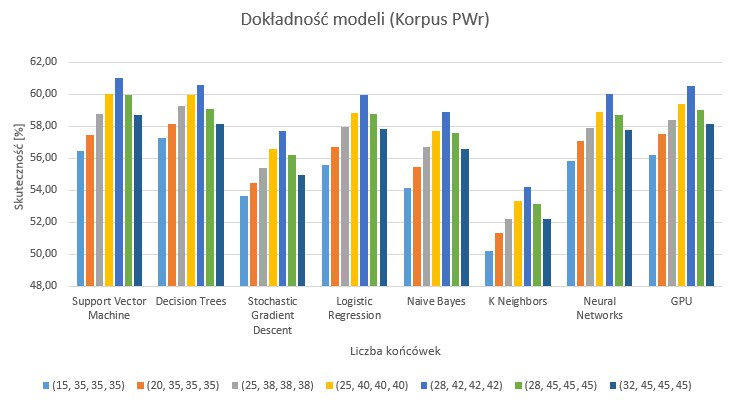
\includegraphics[width=\linewidth]{charts/korpuspwrwykres}
	\label{Rysunek}
	\caption{Skuteczność modeli -- korpus PWr.}
\end{figure}

\begin{figure}[!htbp]
	\centering
	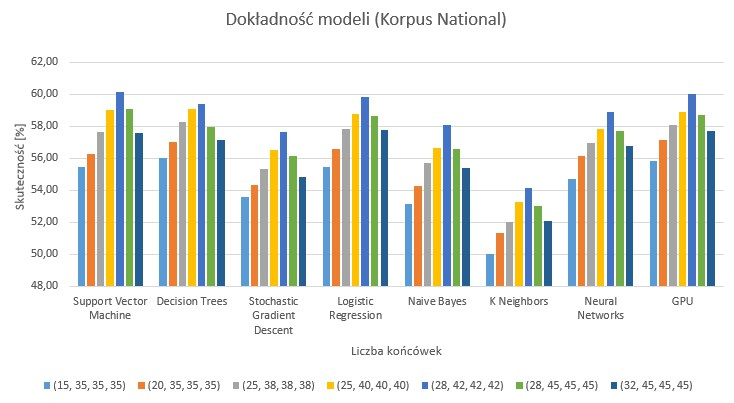
\includegraphics[width=\linewidth]{charts/korpusnationalwykres}
	\label{Rysunek}
	\caption{Skuteczność modeli -- korpus National.}
\end{figure}

\newpage
\subsection{Pomiary czasów uczenia}

\begin{table}[H]
	\centering
	\caption{Pomiary czasów uczenia.}
	\smallskip
	\begin{tabular}{lcc}
		\toprule
		\textbf{Nazwa algorytmu} & \textbf{Korpus uczący PWr (h:m:s)} &  \textbf{Korpus uczący national (h:m:s)} \\
		\midrule
		Support Vector Machine & 2:05:03 & 45:46:28 \\
		Decision Trees & 0:00:30 & 0:02:24 \\
		Stochastic Gradient Descent & 0:00:29 & 0:02:09 \\
		Logistic Regression & 0:01:02 & 0:05:41 \\
		Naive Bayes & 0:00:21 & 0:01:51 \\
		K Neighbors & 0:00:23 & 0:01:49 \\
		Neural Networks & 0:35:20 & 2:21:40 \\
		\bottomrule
	\end{tabular}
\end{table}


Pomiar czasowy wykonany na procesorze Intel(R) Core(TM) i5-2540M CPU @ 2.60GHz.


\newpage
\subsection{Pomiary czasów klasyfikacji}

Pomiary czasów klasyfikacji przeprowadzono na próbie 10 zbiorów tekstów zawierających kolejno od 10 do 100 wyrazów. Wyniki rozdzielono na osobne wykresy przedstawiające odpowiednio klasyfikatory nauczone na korpusie PWr oraz na korpusie podmilionowym.

Zauważyć można, iż na pierwszym wykresie przedstawiającym korpus PWr, najdłuższym czasem klasyfikacji wyróżnił się ten wykorzystujący kartę graficzną, osiągając przy 100 wyrazach czas 11.381 s. Dwukrotnie lepszy czas osiągnął algorytm \texttt{SVM}, osiągając 4.167 s. Trzecim, dziecięciokrotnie szybszym od pierwszego był algorytm K Neighbors -- 1.109 s. Reszta algorytmów może się pochwalić bardzo niskimi czasami, rzędu setnych sekundy, dlatego też na wykresie są prawie niewidoczne.

\begin{figure}[!htbp]
	\centering
	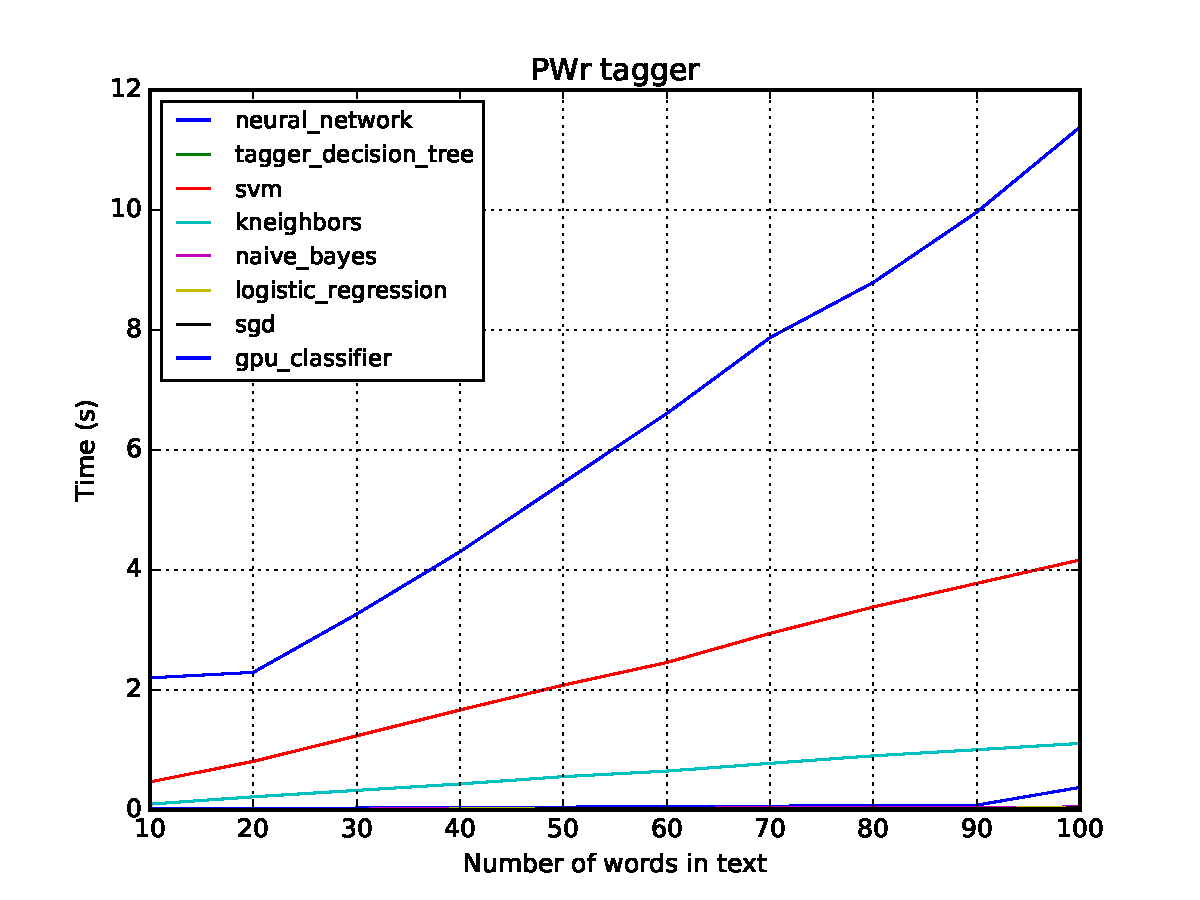
\includegraphics[scale=0.8]{charts/czasy_pwr.pdf}
	\label{Rysunek}
	\caption{Czasy klasyfikacji w zależności od ilości słów w tekście -- korpus PWr.}
\end{figure}

W przypadku korpusu podmilionowego sytuacja jest bardzo podobna z tą różnicą, iż pominięty został algorytm bazujący na karcie graficznej albowiem nie można go było uruchomić na udostępnionej maszynie testowej z powodu niewystarczającej ilości pamięci operacyjnej.

\begin{figure}[!htbp]
	\centering
	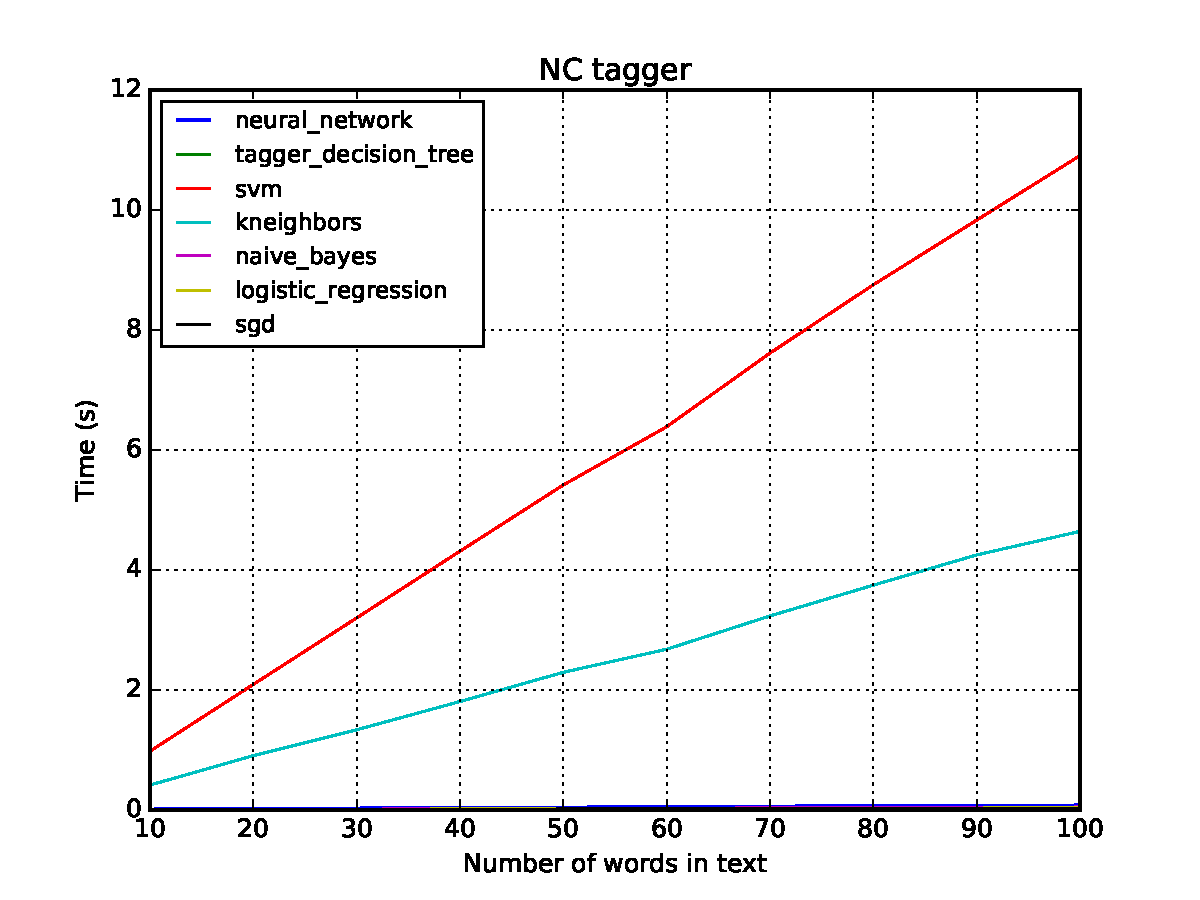
\includegraphics[scale=0.8]{charts/czasy_nc.pdf}
	\label{Rysunek}
	\caption{Czasy klasyfikacji w zależności od ilości słów w tekście -- korpus National.}
\end{figure}
